%
%  For more information, please see: http://software.sci.utah.edu
% 
%  The MIT License
% 
%  Copyright (c) 2004 Scientific Computing and Imaging Institute,
%  University of Utah.
% 
%  License for the specific language governing rights and limitations under
%  Permission is hereby granted, free of charge, to any person obtaining a
%  copy of this software and associated documentation files (the "Software"),
%  to deal in the Software without restriction, including without limitation
%  the rights to use, copy, modify, merge, publish, distribute, sublicense,
%  and/or sell copies of the Software, and to permit persons to whom the
%  Software is furnished to do so, subject to the following conditions:
% 
%  The above copyright notice and this permission notice shall be included
%  in all copies or substantial portions of the Software.
% 
%  THE SOFTWARE IS PROVIDED "AS IS", WITHOUT WARRANTY OF ANY KIND, EXPRESS
%  OR IMPLIED, INCLUDING BUT NOT LIMITED TO THE WARRANTIES OF MERCHANTABILITY,
%  FITNESS FOR A PARTICULAR PURPOSE AND NONINFRINGEMENT. IN NO EVENT SHALL
%  THE AUTHORS OR COPYRIGHT HOLDERS BE LIABLE FOR ANY CLAIM, DAMAGES OR OTHER
%  LIABILITY, WHETHER IN AN ACTION OF CONTRACT, TORT OR OTHERWISE, ARISING
%  FROM, OUT OF OR IN CONNECTION WITH THE SOFTWARE OR THE USE OR OTHER
%  DEALINGS IN THE SOFTWARE.
%


%%%%%%%%%%  Figures used in this file %%%%%%%%%%%%%%%%%%%%%%%%%%%%%%%%
%% The basic viewer window
%begin{latexonly}
\newcommand{\viewerwindow}{%
  \centerline{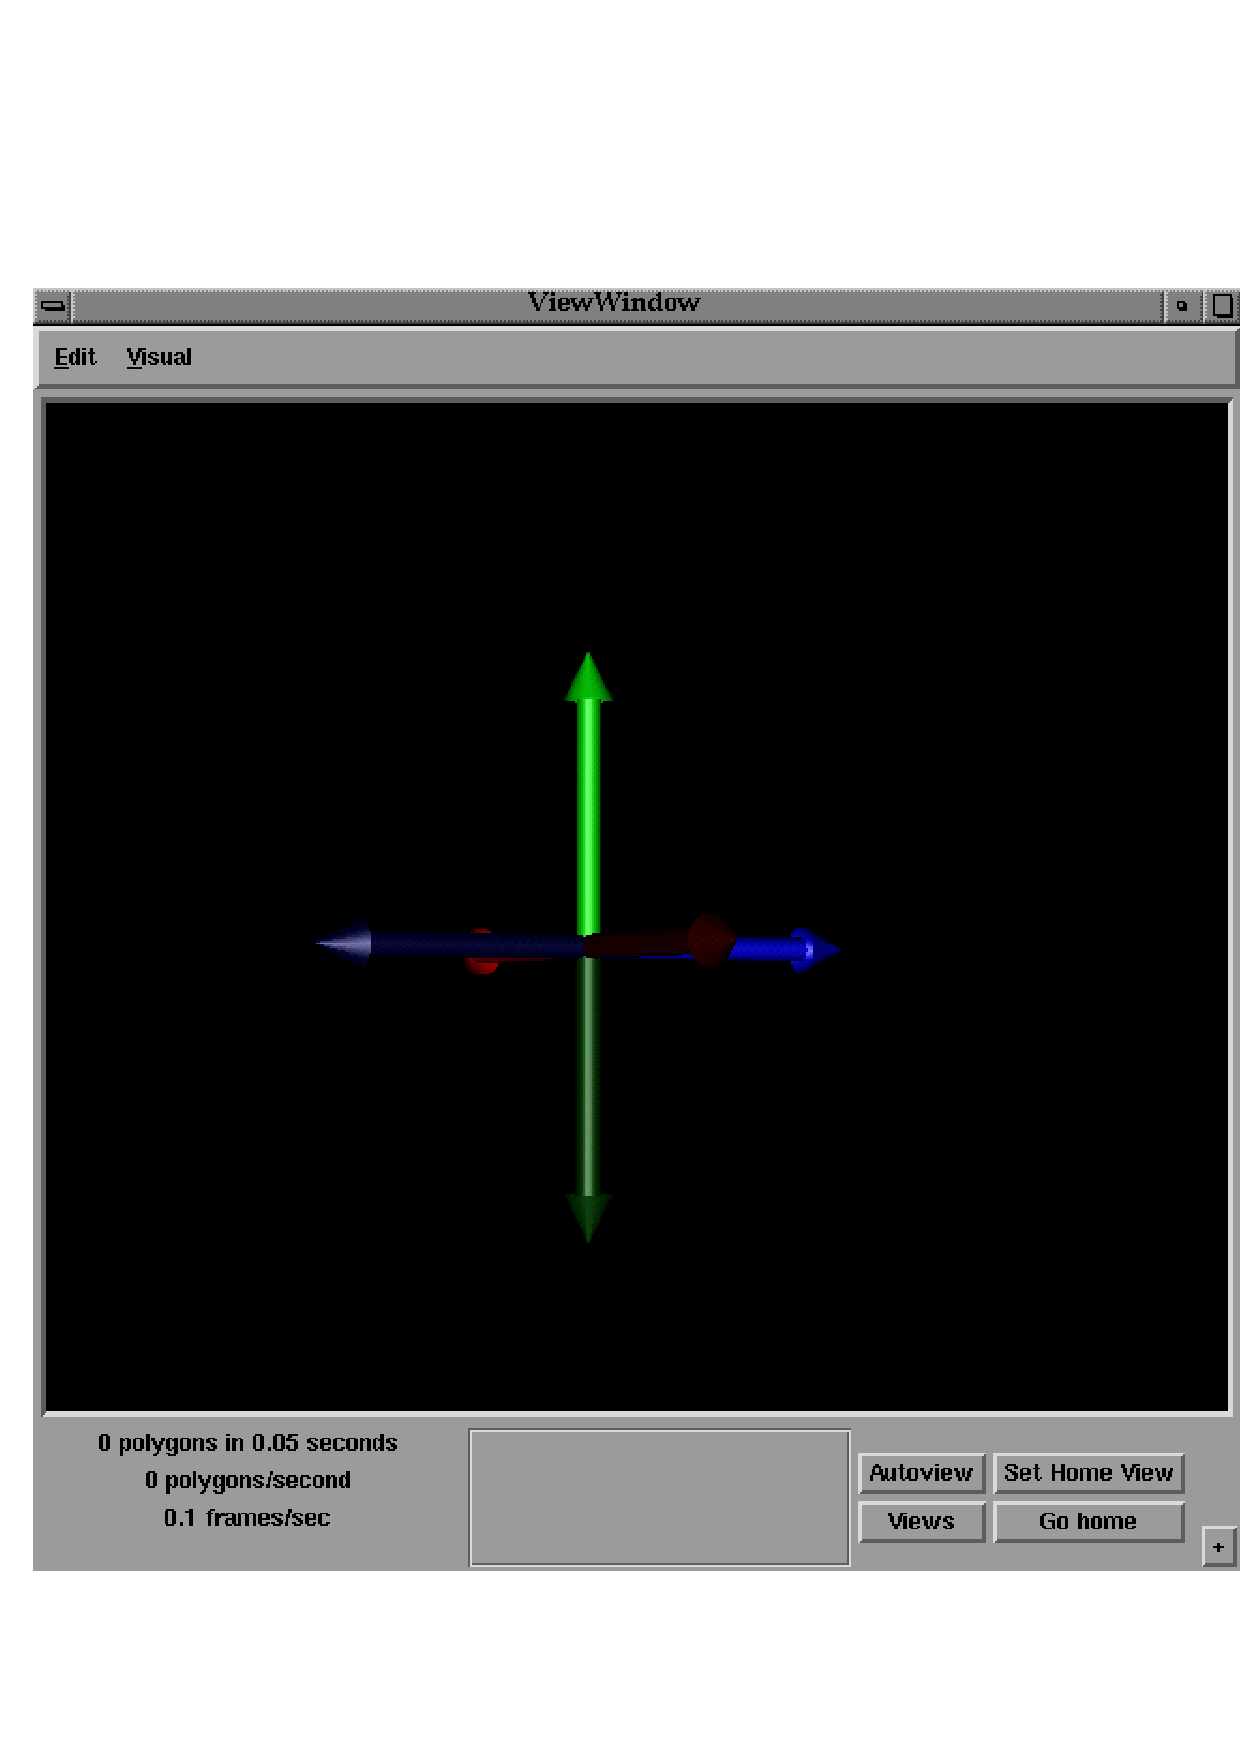
\includegraphics[bb=0 0 491 501,height=4in]
    {Figures/viewwindow.eps.gz}}
}
%end{latexonly}
\begin{htmlonly}
  \newcommand{\viewerwindow}{%
    \htmladdimg[alt="module"]{../Figures/viewwindow.gif}
  }
\end{htmlonly}

%% View of the extended viewer window
%begin{latexonly}
\newcommand{\extendedwindow}{%
  \centerline{\includegraphics[bb=0 0 602 420,height=4in]
    {Figures/viewbottom.eps.gz}}
}
%end{latexonly}
\begin{htmlonly}
  \newcommand{\extendedwindow}{%
  \htmladdimg[alt="extended view window"]{../Figures/viewbottom.gif}}
\end{htmlonly}

%% Point widget image
%begin{latexonly}
\newcommand{\pointwidget}{%
  \centerline{\includegraphics[bb=0 0 230 222,height=2in]
    {Figures/widget-point.eps.gz}}
}
%end{latexonly}
\begin{htmlonly}
  \newcommand{\pointwidget}{%
    \htmladdimg[alt="pointwidget"]{../Figures/widget-point.gif}
  }
\end{htmlonly}

%% Rake widget image
%begin{latexonly}
\newcommand{\rakewidget}{%
  \centerline{\includegraphics[bb=0 0 457 340,height=2in]
    {Figures/widget-gauge.eps.gz}}
}
%end{latexonly}
\begin{htmlonly}
  \newcommand{\rakewidget}{%
    \htmladdimg[alt="rakewidget"]{../Figures/widget-gauge.gif}
  }
\end{htmlonly}

%% Frame widget image
%begin{latexonly}
\newcommand{\framewidget}{%
  \centerline{\includegraphics[bb=0 0 328 268,height=2in]
    {Figures/widget-frame.eps.gz}}
}
%end{latexonly}
\begin{htmlonly}
  \newcommand{\framewidget}{%
  \htmladdimg[alt="framewidget"]{../Figures/widget-frame.gif}}
\end{htmlonly}

%% Box widget image
%begin{latexonly}
\newcommand{\boxwidget}{%
  \centerline{\includegraphics[bb=0 0 458 342,height=2in]
    {Figures/widget-box.eps.gz}}
}
%end{latexonly}
\begin{htmlonly}
  \newcommand{\boxwidget}{%
    \htmladdimg[alt="boxwidget"]{../Figures/widget-box.gif}
  }
\end{htmlonly}

%% Ring widget image
%begin{latexonly}
\newcommand{\ringwidget}{%
  \centerline{\includegraphics[bb=0 0 507 467,height=2in]
  {Figures/widget-ring.eps.gz}}
}
%end{latexonly}
\begin{htmlonly}
  \newcommand{\ringwidget}{%
    \htmladdimg[alt="ringwidget"] {../Figures/widget-ring.gif}
  }
\end{htmlonly}

%% Record movie dialog window
%begin{latexonly}
\newcommand{\recordmoviewin}{%
  \centerline{\includegraphics[bb=0 0 176 183]
    {Figures/record_movie_win.eps.gz}}
}
%end{latexonly}
\begin{htmlonly}
  \newcommand{\recordmoviewin}{%
  \htmladdimg[alt="Movie Recording
  Dialog"]{../Figures/record_movie_win.gif}
}
\end{htmlonly}

%%%%%%%%%%%%%%%%%%%%%%%%%%%%%%%%%%%%%%%%%%%%%%%%%%%%%%%%%%%%%%%%%%%%%%
\newcommand{\graphics}{\emph{Graphics}}

\chapter{Visualization}
\label{ch:viewer}
\index{Viewer@\viewer{}}

This section describes the most frequently used \sr{} module,
the \viewer{}, which displays interactive graphical
output to the computer screen.  The \viewer{} is used any time the user
wants to see a geometry or spatial data. The \viewer{} also provides access to
many simulation parameters and controls, and indirectly initiates new
iterations of  simulation steps, which is important for computational
steering (see \secref{Computational Steering}{sec:con-steering}).
Multiple \viewer{} windows can be created.  Each viewer window is
independent of the others.

This section begins with an overview of the \viewer{} window and its
controls, then describes the options and variations.

\section{Anatomy of the \viewer{} Window}
\label{sec:viewer-anatomy} 
\index{Viewer@\viewer{}!anatomy}

The \viewer{} window contains two main areas.  The upper portion,
which displays graphics and is called the \graphics{} window, and the
lower portion where the majority of control buttons are found.
Figure~\ref{fig:viewwindow} contains an example of a \viewer{} window.
In the \graphics{} window, viewing is controlled by the mouse, mouse
buttons, and various modifier keys (shift/control/alt).  In the lower
window there are several buttons and sliders. Their function is
described in this section.

\begin{figure}[htb]
  \begin{makeimage}
  \end{makeimage}
  \viewerwindow
%    \framebox{\parbox[3in]{\columnwidth}{The\dotfill Figure\\
%    \vspace{2in}\\
%    With some \dotfill dummy text}}
  \caption{\label{fig:viewwindow} The default \viewer{} window in \SR{}}
\end{figure}


The visible controls along the bottom of the \viewer{} window set default
configurations as follows:
%
\begin{description}
  \buttondesc{Autoview} Restores the display to a default
  condition.  Useful when some combination of settings result in
  objects disappearing from the view window.
  
  \buttondesc{Set Home View} Captures the setting of the current view
  so the user can return to it later by clicking the ``Go home''
  button.

  \buttondesc{Go home} Restores the current home view.
  
  \buttondesc{Views} Lists a number of standard viewing angles
  and orientations.  The view directions align with the Cartesian axes
  of the objects, and the ``Up vector'' option sets the orientation of
  the objects when viewed along the selected axis.
\end{description}

The display's rendering speed is shown in the lower left corner of the
\viewer{}'s control window.  

More controls can be revealed by clicking the
\latexhtml{\fbox{+}}{\button{[+]}} button in the lower right corner of
the \viewer{} window (see \secref{Extended Control Window}
{sec:view-control} for a description of extended controls).


\subsection{Menus}
\index{Viewer@\viewer{}!menus}

The \viewer{} window's menu bar contains the \menu{File}, \menu{Edit},
and \menu{Visual} menus and the \guibutton{NewViewer} button.

\begin{description}
  \menudesc{File} The \menu{File} menu contains the following items:

  \begin{description}
    \menuitemdesc{Save Image...} Saves the contents of the \viewer{}
    window as an image to a file.  A dialog prompts the user for a
    file name, an image format, and an image size.
    
    \menuitemdesc{Record Movie...} Saves the contents of the \viewer{}
    window as a movie.  See \secref{Recording
      Movies}{sec:recordmovies} for more information.
  \end{description}
  
  % All of the items below need further explication.
  \menudesc{Edit} The \menu{Edit} menu contains the following items:
  \begin{description}
    \menuitemdesc{View/Camera...} Edit eye point, look
    at point, up vector, and field of view settings.

    \menuitemdesc{Light Sources...} Edit light sources, colors, and
    brightness.  Light source locations are specified relative to the
    camera.  Alternatively, using module \module{AddLight} (category
    Visualization in the \sr{} package), light sources can be specified
    as objects in the scene.

    \menuitemdesc{Background...} Change the \viewer{}
    window's background color.

    \menuitemdesc{Clipping Planes...} Edit the orientation and visibility
    of clipping planes.

    \menuitemdesc{Point Size...} Increase or decrease the size of points.

    \menuitemdesc{Line Width...} Increase or decrease the width of lines.
    
    \menuitemdesc{Polygon Offset...} Set the polygon offset parameter.
    This parameter is used to improve rendering of coplanar
    polygons, lines, and points by offsetting polygons (by a small
    amount) from other objects.

    \menuitemdesc{Scene Materials...} Edit scene material properties.
  \end{description}

  \menudesc{Visual} Allows the user to select different
  graphics hardware settings that are available on the workstation.
  The list is ordered heuristically from most to least useful.

  \menudesc{NewViewer} \guibutton{NewViewer} creates a new \viewer{}
  window when pressed.  Each viewer window is independent of other
  viewer windows.
\end{description}

\section{Recording Movies}
\label{sec:recordmovies} 
\index{movies}

\begin{figure}[htb]
  \begin{makeimage}
  \end{makeimage}
  \recordmoviewin
  \caption{\label{fig:recordmoviewin} Movie Recording Window}
\end{figure}

The \viewer{}'s recording control window controls movie recording.
Figure~\ref{fig:recordmoviewin} shows the recording control window.
Select \menuitem{Record Movie\dots} from the \viewer{} window's
\menu{File} menu to show the movie control window.

\sr{} makes a movie by recording the content of the \viewer{} window
each time the \viewer{} window is redrawn.  The width and height of
each frame is the same size as the width and height of the \viewer{}
control window.  The width and height of each frame may be changed by
clicking button \guibutton{Resize} and typing width and height values
into the resize text boxes---this must be done before recording the
movie.

A movie can be saved as a series of PPM frames, one frame per
file,  or as an MPEG file.

When saving a movie as a series of PPM files, the files are named
according to the C-style format string in the the \guilabel{Name:}
text box and the initial frame number in the \guilabel{Frame:} text
box.  The frame number is formatted according to the conversion
specification introduced by the percent '\%' character.  For example,
if \guilabel{Name:} is \icode{movie.\%04d} and \guilabel{Frame:} is 1
then the following series of file names are generated:
\filename{movie.0001}, \filename{movie.0002}, \ldots,
\filename{movied.1000} for a PPM movie with one thousand frames.

When recording an MPEG movie, the \guilabel{Name:} text box contains
the name of the MPEG file.

Click radio button \guibutton{PPM} to begin a PPM recording.  Click
button \guibutton{Mpeg} to begin an MPEG recording.  Click button
\guibutton{Stop Recording} to end a movie.


\section{Mouse Control in the \viewer{} Window}
\label{sec:view-mouse} 
\index{Viewer@\viewer{}!mouse controls}

The \viewer{}'s mouse controls are extensive and flexible.  The
resulting action depends on the choice of mouse button, how the mouse
is moved and simultaneously pressed control keys.  The descriptions in
Tables~\ref{tab:view-mouse} and~\ref{tab:view-unicam} may seem
complicated, but with practice, use of the mouse becomes intuitive.


\begin{table}[htb]
\begin{center}
  \begin{tabular}{|l|l|p{5in}|} \hline
    \multicolumn{3}{|c|}{\large Mouse Controls}\\ \hline \hline 
    \multicolumn{1}{|c|}{Control Key} & 
    \multicolumn{1}{|c|}{Button} & 
    \multicolumn{1}{|c|}{Action}\\ \hline
None & Left & Translate scene \\
     & Middle & \begin{raggedleft} Rotate scene about its center on an arc
    ball that surrounds it; rotation direction is a function of the
    initial mouse location so try different sites and note the
    response. \end{raggedleft}\\  
     & Right & Zoom or scale scene (downwards and to the right increases
     size, upwards or to the left decreases size) \\ \hline
Shift & Left & Select and move a widget in the display \\
      & Middle & Toggle through the modes for a widget \\
      & Right & Pop up a widget information window \\ \hline
Control & Left & Translate in the Z-direction, \ie{} zoom in and out of the
    screen (down moves closer, up further away).  Moving left and
    right increases the ``throttle'' of the Z-direction motion.  If
    the cursor is over a point on an object when clicked, this point
    becomes the center of the screen for translation.\\ 
      & Middle & Rotate the camera view about the eye point (using arcball
    motion). \\ 
      & Right & Unicam movement (see Table~\ref{tab:view-unicam})\\ \hline
\end{tabular}
\caption{\label{tab:view-mouse} Mouse controls for the \viewer{}}
\end{center}
\end{table}

\bigskip

\begin{table}
\begin{center}
\begin{tabular}{|l|l|p{3in}|} \hline
    \multicolumn{3}{|c|}{\large Unicam movement (Control key and right mouse
    button} \\ \hline \hline
    \multicolumn{1}{|c|}{Initial mouse location} & 
    \multicolumn{1}{|c|}{Action} & \\ 
    \hline
    Near edge of display & Rotate objects on the arc ball & \\
    Near the objects & Following behavior: & \\
    \hline
    & \multicolumn{1}{|c|}{Initial mouse movement} & 
    \multicolumn{1}{|c|}{Action}\\ \hline
    & Horizontal & Pan objects \\ 
    & Vertical & Zoom and pan: down = zoom in, up = zoom
    out, left and right= pan left and right) \\
    & None & Set rotation point for subsequent arc ball rotation.\\
    \hline
\end{tabular}
\caption{\label{tab:view-unicam} Autocam mouse controls in the \viewer{}}
\end{center}
\end{table}



\section{Extended Control Window}
\label{sec:view-control} 
\index{Viewer@\viewer{}!extended controls}

Clicking on the \button{[+]} button in the lower right corner of the
default \viewer{} window expands to reveal an extended panel of
control buttons as shown in Figure~\ref{fig:extviewwindow}.  Note that
\button{[+]} changes to \button{[-]}.  Clicking on the \button{[-]}
button hides the extended control panel.  The following sections
describe the control options available in the extended control
window.

\begin{figure}[htb]
  \begin{makeimage}
  \end{makeimage}
  \extendedwindow
%    \framebox{\parbox[3in]{\columnwidth}{The\dotfill Figure\\
%    \vspace{2in}\\
%    With some \dotfill dummy text}}
  \caption{\label{fig:extviewwindow} The lower portion of extended
    \viewer{} window in \SR{}} 
\end{figure}


\subsection{Rendering Controls}
\label{sec:view-rendering} 
\index{Viewer@\viewer{}!rendering}

The left part of the extended \viewer{} window contains global
rendering settings.  Objects can override global settings.  See
\secref{Object Selection and Settings}{sec:object-settings} for making
object specific settings.

The rendering options are:

\begin{description}
  \descitem{Lighting} Toggles whether or not the \viewer{} applies
  lighting to the display.  Objects without lighting have a constant
  color.
        
  \descitem{Fog} Draws objects with variable intensity based on their
  distance from the user, also known as ``depth cueing''.  Close
  objects appear brighter while more remote objects fade gradually
  into the background as a function of distance from the front.
  
  \descitem{BBox} Toggles whether the \viewer{} draws the selected
  objects in full detail, or as a simple bounding box.
  
  \descitem{Use Clip} Applies up to six clipping planes to the
  display.  To control the clipping plane locations, use the ``Edit
  -\ra{} Clipping Planes'' menu at the top of the \viewer{} window.
  
  \descitem{Back Cull} Displays only the forward facing facets of any
  surface objects in the display.
  
  \descitem{Display List} Cache the list of objects to be displayed.
  This option accelerates rendering when the content of the display
  does not change.

  \descitem{Wire} Show only the wire mesh of objects.

  \descitem{Flat} Draw each facet with a constant color.

  \descitem{Gouraud} Linearly interpolate color across facets. 
\end{description}

The right column of the extended \viewer{} window contains controls
for displaying the axes and creating stereoscopic rendering.  

\subsection{Object Selection and Settings}
\label{sec:object-settings}

The middle panel of the extended \viewer{} window lists objects
displayed in the \viewer{} window.  Each list entry consists of the
following items (from left to right):

\begin{itemize}
\item Selection button.  An object is selected when the selection
  button is depressed.  The \viewer{} window only displays selected
  objects.
\item An object's name.
\item A \menu{Options...} pop-up menu.  The \menu{Options...} menu
  controls object specific rendering settings.  If item \menuitem{Use
    Global Controls} is set then object specific settings are ignored
  and global rendering settings are used.  Rendering settings
  are discussed in \secref{Rendering Controls}{sec:view-rendering}.
\end{itemize}


\subsection{Miscellaneous Settings}

The right part of the of the extended \viewer{} window contains the
following settings:

\begin{description}
\descitem{Show Axes} Toggles the display of coordinate axes centered at
coordinate (0, 0, 0).

\descitem{Orientation} Toggles the display of orientation axes.
Orientation axes are displayed in the upper right corner of the
\viewer{} window.

\descitem{Ortho View} Toggles between perspective and orthographic views.

\descitem{Stereo} Toggles stereo view on and off.  Stereo view
requires hardware LCD glasses synchronized with the display, so
visibility in each eye coincides with the display of the appropriate
view.

\descitem{Fusion Scale} Controls left and right eye image separation
for stereo viewing.  Allows the user to establish a separation that is
suited to facial anatomy and distance from the screen.

\end{description}


\section{Control Widgets}
\label{sec:view-widgets}
\index{Viewer@\viewer{}!widgets}


\SR{} supports powerful display widgets.  Examples of widget
capabilities include managing cutting surfaces colored according to
the local data values, displaying streamlines in vector fields, or
selecting sub-volumes within the display area for further
manipulation.
 
\sci{} has made interaction with widgets as consistent as
possible. For example, controlling parameters is usually done by
clicking and dragging on a cylindrical ``collar'' or a sphere element
of the widget. Note that a single widget can have more than one
purpose depending on the context in which it exists. The Rake widget,
for example, selects a clipping or display plane through a
three-dimensional object, and sets the seed points for a streamline
module.

This section describes the widgets available within \SR{} and \BIOPSE{}.
 
\subsection{Point Widget}
\label{sec:view-pointwidget} 

\begin{figure}[htb]
  \begin{makeimage}
  \end{makeimage}
  \pointwidget
  \caption{\label{fig:pointwidget} The point widget for probing fields}
\end{figure}

\paragraph{Appearance} The Point widget consists of a sphere (see Figure~\ref{fig:pointwidget}).

\paragraph{Purpose} The primary purpose of the Point Widget is to
select and retrieve information about a point, for example when
probing a field.

\paragraph{Controls} Clicking and dragging the sphere moves the point
widget to a new location.

\subsection{Rake Widget}
\label{sec:view-rakewidget} 

\begin{figure}[htb]
  \begin{makeimage}
  \end{makeimage}
  \rakewidget
%    \framebox{\parbox[3in]{\columnwidth}{The\dotfill Figure\\
%    \vspace{2in}\\
%    With some \dotfill dummy text}}
  \caption{\label{fig:rakewidget} The rake widget for setting location and
    density of seed points}
\end{figure}

\paragraph{Appearance} The Rake
Widget has an orientation, length, and value (see Figure~\ref{fig:rakewidget}). It consists of two spheres (A) connected by a cylinder (B) with a
small slider collar (C) on the cylinder.  There are also small resize
cylinders (D) extending from the spheres.

\paragraph{Purpose} The primary use of the Rake Widget is to set the
location and density of streamlines emerging from the long cylinder.  It
can also be used as a more general purpose three-dimensional slider, or a
source for a stream surface. 

\paragraph{Controls} Clicking and dragging either sphere changes the widget's orientation.  Dragging either of the resize
cylinders causes the size of the widget to change, and dragging any point on
the main cylinder moves the whole widget without any change in orientation.
Dragging the slider collar changes the associated value, typically the
density of seed points for a streamline source.

\subsection{Frame Widget}
\label{sec:view-framewidget} 

\begin{figure}[htb]
  \begin{makeimage}
  \end{makeimage}
  \framewidget
%    \framebox{\parbox[3in]{\columnwidth}{The\dotfill Figure\\
%    \vspace{2in}\\
%    With some \dotfill dummy text}}
  \caption{\label{fig:framewidget} The Frame Widget}
\end{figure}


\subsubsection{Appearance} The
Frame Widget (see Figure~\ref{fig:framewidget}) consists of four cylinders connected in a rectangle.  In
the middle of each cylinder there is a sphere (B), from which
a resize cylinder extends (C).

\subsubsection{Purpose} The Frame Widget is primarily used for image
plane definition, defining stream volumes, and as a "tie dye'' similar to
the Ring Widget described in \secref{Ring Widget}{sec:view-ringwidget}.

\subsubsection{Controls} Dragging a sphere rotates the widget about its center. Dragging on a resize cylinder extends or contracts the rectangle.
Dragging any cylinder drags the entire widget through space.


\subsection{Box Widget}
\label{sec:view-boxwidget} 

\begin{figure}[htb]
  \begin{makeimage}
  \end{makeimage}
  \boxwidget
%    \framebox{\parbox[3in]{\columnwidth}{The\dotfill Figure\\
%    \vspace{2in}\\
%    With some \dotfill dummy text}}
  \caption{\label{fig:boxwidget} The boxwidget for selecting sub-volumes}
\end{figure}

\subsubsection{Appearance} The Box
Widget (see Figure~\ref{sec:view-boxwidget}) consists of twelve 
connected cylinders (A) to form a hexahedral box (B) (three-dimensional
rectangle).  In the middle of each face of the box is a sphere with a protruding cylinder (C) providing resize control.

\subsubsection{Purpose} The Box Widget is primarily used to select a
subvolume of the workspace for further manipulation (\eg{} volume
rendering, isosurfaces, streamlines, mesh adaption) where the faces of the
widget act as orthogonal clipping planes.

\subsubsection{Controls} Clicking on and dragging a sphere rotates
the widget about its center without changing the position of the center.
Clicking on and dragging any resize handle
% What do these look like??
causes the associated face to extend without changing its orientation.
Dragging a cylinder causes the entire widget to move without changing its
orientation.

\subsection{Ring Widget}
\label{sec:view-ringwidget} 

\begin{figure}[htb]
  \begin{makeimage}
  \end{makeimage}
  \ringwidget
%    \framebox{\parbox[3in]{\columnwidth}{The\dotfill Figure\\
%    \vspace{2in}\\
%    With some \dotfill dummy text}}
  \caption{\label{fig:ringwidget} The ring widget for selecting
    cutting/projection planes}
\end{figure}


\subsubsection{Appearance} The Ring
Widget (see Figure~\ref{sec:view-ringwidget}) consists of a ring (A)
with four embedded spheres (B), each with a resize cylinder
attached (D).  Between two of the spheres is a sliding collar (C).
One of the resize cylinders has a special material property (typically
a different color from the other cylinders) to indicate that it is the
``halfway point'' for the slider (E).

\subsubsection{Purpose} The Ring Widget is primarily used to set the
density of streamlines emerging from the ring. The ring serves as a set of
seed points from which streamlines emerge. The Ring Widget can 
serve as a three-dimensional angle gauge, as a source for multiple
streamlines throughout its surface, as a source for a stream surface from
the outer ring, and as a source for a stream volume.  The Ring Widget can 
also be used as a color sheet, or ``tie dye'', in which the surface is colored as 
a function of the scalar value of the field at each point.

\subsubsection{Controls} Clicking and dragging the slider collar along the
ring changes the density of the seed points or some other related
parameter.  Dragging the spheres controls the orientation of the Ring
Widget, while moving the resize cylinders change the radius of the Ring
Widget about its center.  Dragging any other point on the ring moves the
ring in space without changing its radius or orientation.
